\documentclass[11pt,a4paper]{article}

\usepackage{titling}
\usepackage[hidelinks]{hyperref}
\usepackage{graphicx}
\usepackage{grffile}
\usepackage{float}
\usepackage{geometry}

\newcommand{\subtitle}[1]{
  \posttitle{
    \par\end{center}
    \begin{center}\large#1\end{center}
    \vskip0.5em}
}

\begin{document}
\title{Benchmark Service Functional Requirements Documentation}
\subtitle{ Git: \url{https://github.com/CodingInfinity/Benchmark-Service-Documentation} \\ GitHub Organisation: \url{https://github.com/CodingInfinity}}
\begin{figure}
			\centering
			
\includegraphics[height=230px]{../Images/CodingInfinity.png}
\end{figure}
\author{
	\textbf{The Client:} \\
	Ms Vreda Pieterse  \\
	Department of Computer Science \\
	University Of Pretoria
	\\
	\\
	\textbf{The Team:} \\
	Andrew Broekman		\emph{11089777}	\\
	Brenton Watt		\emph{14032644}	\\
	Fabio Loreggian		\emph{14040426}	\\
	Reinhardt Cromhout	\emph{14009936}	\\
}
\date{\textbf{May 2016}}

\maketitle
\thispagestyle{empty}
\pagebreak

\tableofcontents
\pagebreak

\section{Introduction}
\subsection{Background in Benchmarking}
There are many cases in the industry, in research and in education where benchmarking of
a software product is important. In industry benchmarks can be used to ensure that software
performance is acceptable. In the competitive commercial world, benchmarks can serve to inform
buyers of comparative performance of competing products. The benchmarking forms an integral
part of research related to the development of new algorithms and techniques as well as the refinement
and optimization of existing operations. Algorithm and data structure benchmarks can be applied
as a very useful teaching tool for students to review the notions of space and time complexity.

It is strange that although benchmarking seem to be a very common and useful application, very few benchmarking tools or services are available. Those that are available requires intricate configuration that may be beyond the reach of the developers, researchers,
teachers and students who would like to use them. The development of a benchmarking service which can be used in a generic way would therefore be welcomed by a large
potential user base.

\subsection{Our System}
Our system will consist of \textbf{Five} Modules namely User Managment, Benchmarking Service, Reporting, Notifications and Test Data.\\
The following modules may contain, and are not limited to the follwing, as according to Agile Process.

\subsubsection{User Managment}
This module consists of:
\begin{itemize}
  \item User Admin
  \item User Signup
  \item User Login
  \item User Profile Managment
\end{itemize}

\subsubsection{Benchmarking Service}
This module consists of:
\begin{itemize}
  \item Backend to run the user program
  \item Watcher service to monitor the program.
\end{itemize}

\subsubsection{Reporting}
This module consists of:
\begin{itemize}
  \item Reporting of a Benchmarking instance
  \item Comparing multiple Benchmakrs
  \item Exporting to report pdf
\end{itemize}

\subsubsection{Notifications}
This module consists of:
\begin{itemize}
  \item Notifying the user that there Benchmark is complete
\end{itemize}

\subsubsection{Test Data}
This module consists of:
\begin{itemize}
  \item Providing basic template data
  \item Adding data to repository
  \item Generating Test data
  \item Storing Test Data
\end{itemize}


\section{Vision and Objectives}
\subsection{Vision}
There are many cases in the industry, in research and in education where benchmarking of
a software product is important. In industry benchmarks can be used to ensure that soft-
ware performance is acceptable. In the competitive commercial world, benchmarks can
serve to inform buyers of comparative performance of competing products. The bench-
marking forms an integral part of research related to the development of new algorithms
and techniques as well as the refinement and optimization of existing operations. Algo-
rithm and data structure benchmarks can be applied as a very useful teaching tool for
students to review the notions of space and time complexity.\\ \\
There are many cases in the industry, in research and in education where benchmarking of
a software product is important. In industry benchmarks can be used to ensure that soft-
ware performance is acceptable. In the competitive commercial world, benchmarks can
serve to inform buyers of comparative performance of competing products. The bench-
marking forms an integral part of research related to the development of new algorithms
and techniques as well as the refinement and optimization of existing operations. Algo-
rithm and data structure benchmarks can be applied as a very useful teaching tool for
students to review the notions of space and time complexity.


\subsection{Objectives}
The main objectives of the benchmarking service is to provide an integrated platform:
\begin{itemize}
	\item For benchmarking source code from various languages.
	\item For benchmarking various types of software code such as data structures,
        artificial intelligence algorithms, common application code and various 
        other types of software code.
	\item Allowing users to compare the results of various benchmarks.
	\item To ease the management related to the generation, storing, cataloguing 
        of test data and measurements made by the system.
\end{itemize}


\section{Experiment Management}
The \textit{Benchmark Service} module is responsible for monitoring the running
program and gathering data from the instance and generate data, and send it to
the web client for reporting. The monitor will record data such as CPU time,
CPU usage, RAM usage, Network throughput, Overall running time, etc.
\\
\\
The benchmark service then will delete the instance of the running program them
send the data collected to the web serve in order for it to be processed so a
report can be generated. It will store the data in a database. When the benchmarking
is complete, the system will use the notifiaction system to notify the client their
benchmark is complete.


\subsection{Scope}
The scope for the Benchmark Service module is shown in Figure \ref{Benchmark Scope}
\begin{figure}[H]
  \begin{center}
  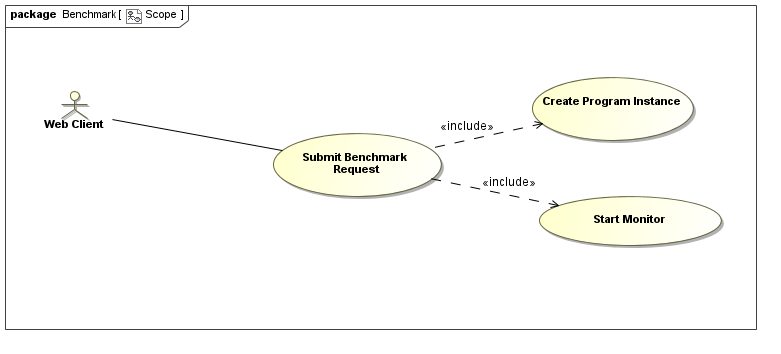
\includegraphics[scale=0.5]{../Diagrams and Charts/Benchmark/Scope.png}
  \caption{Benchmark Scope}
  \end{center}
  \label{Benchmark Scope}
\end{figure}
The scope of the Benchmark Service module include:
\begin{itemize}
	\item Receive a program to run.
  \item Monitor the program instance
  \item Record data
  \item Generate server data for reporting, using the Reporting Module
  \item Store data in database
\end{itemize}

\subsection{Domain Model}
The domain model for the Benchmark Service module is shown in Figure \ref{Benchmark Domain Model}
\begin{figure}[H]
  \begin{center}
  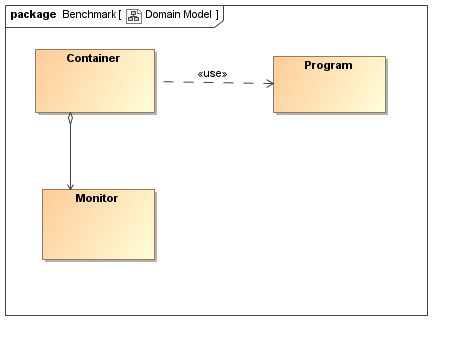
\includegraphics[scale=1.0]{../Diagrams and Charts/Benchmark/Domain Model.png}
  \caption{Benchmark Domain Model}
  \end{center}
  \label{Benchmark Domain Model}
\end{figure}
There will be a container which contains the program to be run, and the monitor to monitor the program instance.\\


\section{Notification}
The \textit{Notification} module is responsible for keeping the user informed 
as to when the benchmarking on their work is done. this is in place because
results will often not be instant due to factors such as queues because of server
load or algorithm needing a large of time to be throughly benchmarked. Once the
benchmarking is completed, the user will be notified by email that they can now
view their results.

\subsection{Scope}
The scope for the users module is shown in Figure \ref{Notifications Scope}
\begin{figure}[H]
	\begin{center}
		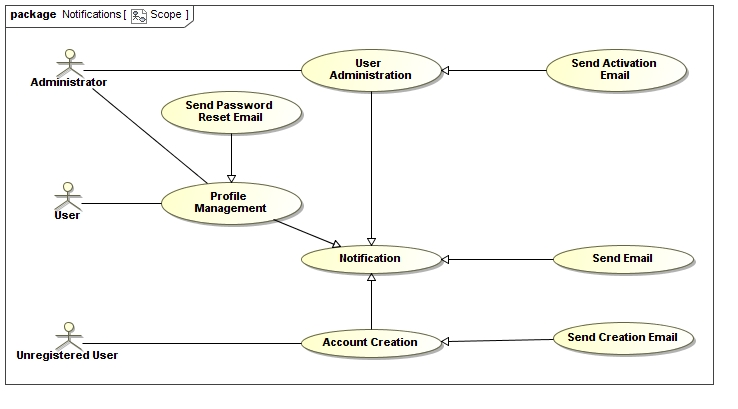
\includegraphics[scale=0.5]{../Diagrams and Charts/Notifications/Scope.jpg}
		\caption{Notifications Scope}
		\label{Notifications Scope}
	\end{center}	
\end{figure}
The scope of the Notification module includes:
\begin{itemize}
	\item sendEmail
	\item sendActivationEmail
	\item sendCreationEmail
	\item sendPasswordResetMail
\end{itemize}

These use cases will be used by the User Management Module to assist with the user
authenication amoung other things. That being said the module provides the
functionality to send emails which can be used by any other module that needs this
functionality.

\subsection{Domain Model}
The domain model for the notifications module is shown in Figure \ref{Notifications Domain Model}
\begin{figure}[H]
	\begin{center}
		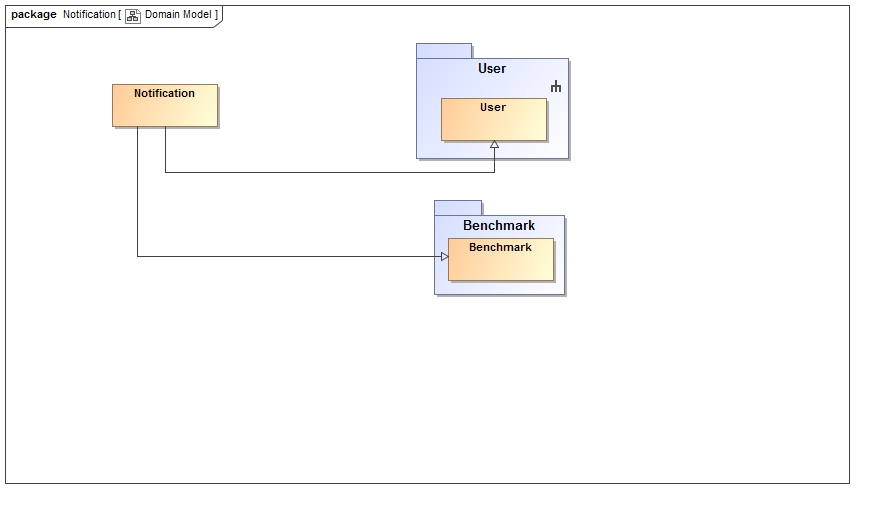
\includegraphics[scale=0.5]{../Diagrams and Charts/Notifications/Domain Model.jpg}  
		\caption{Notifications Domain Model}
		\label{Notifications Domain Model}
	\end{center}	
\end{figure}

\subsection{sendEmail}
Sends an email to a spesific address with a spesified heading and content
provided all the details given are valid.

\subsubsection{Service Contract}
The service contract for the sendEmail use case is shown in Figure \ref{sendEmailServiceContract}
\begin{figure}[H]
	\begin{center}
		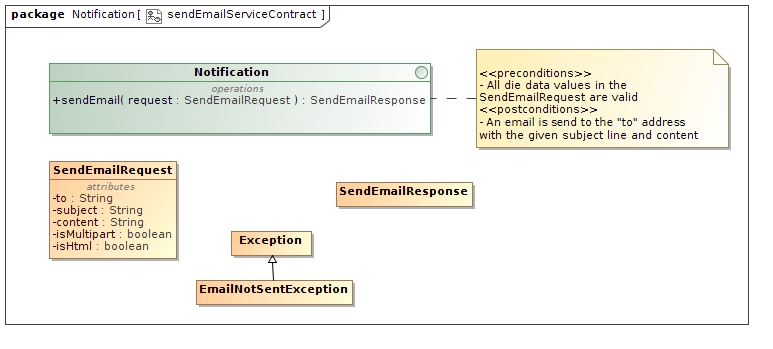
\includegraphics[scale=0.5]{../Diagrams and Charts/Notifications/sendEmailServiceContract.jpg}
		\caption{The service contract for the sendEmail use case}
		\label{sendEmailServiceContract}
	\end{center}	
\end{figure}

The use case sends an email to a spesific address with a spesified heading and content
provided all the details given are valid. If any of the fields in the request object,
particularly the "to" field are not valid the serivce will throw a EmailNotSentException.

\subsubsection{Functional Requirements}
The lower level services required by the sendEmail service to either check the
pre-conditions or address the post-conditions is shown in Figure
\ref{sendEmailFunctionalRequirements}.
\begin{figure}[H]
	\begin{center}
		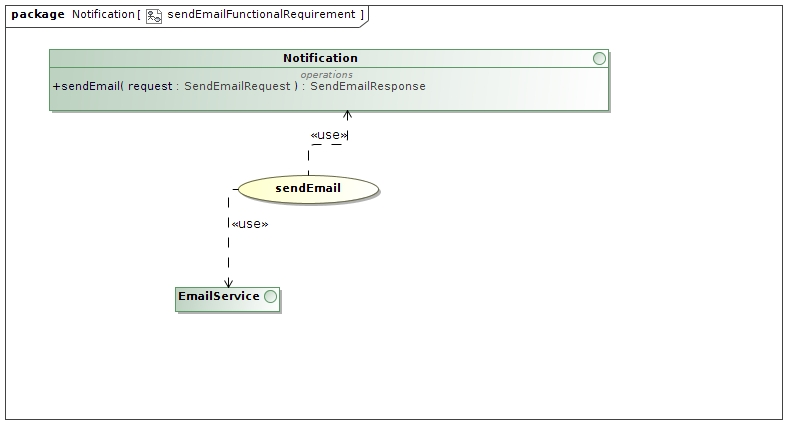
\includegraphics[scale=0.5]{../Diagrams and Charts/Notifications/sendEmailFunctionalRequirement.jpg}
		\caption{The functional requirements for the sendEmail use case}
		\label{sendEmailFunctionalRequirements}
	\end{center}	
\end{figure}

In this case the only service needed by the use case is some form of an email
API.

\subsection{sendActivationEmail}
Used to send a newly created managed user an email regarding the settings of
their password.

\subsubsection{Service Contract}
The service contract for the sendActivationEmail use case is shown in Figure \ref{sendActivationEmailServiceContract}
\begin{figure}[H]
	\begin{center}
		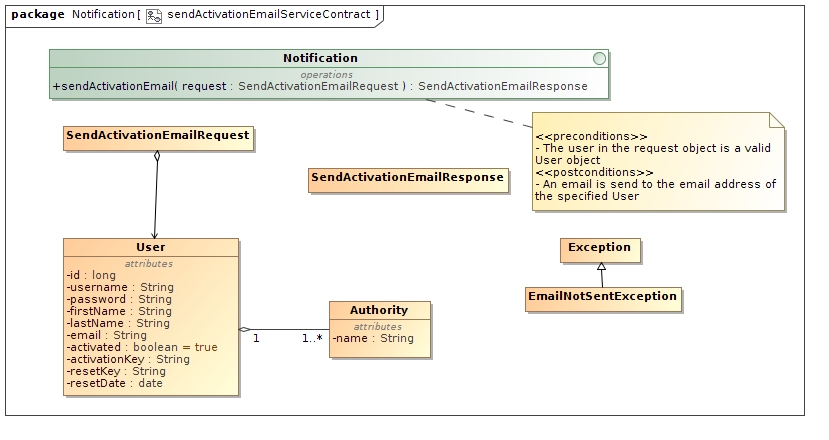
\includegraphics[scale=0.5]{../Diagrams and Charts/Notifications/sendActivationEmailServiceContract.jpg}
		\caption{The service contract for the sendActivationEmail use case}
		\label{sendActivationEmailServiceContract}
	\end{center}	
\end{figure}

The use case sends an email to a spesified User. This email allows the user to
activate his account after it has been created.

\subsubsection{Functional Requirements}
The lower level services required by the sendActivationEmail service to either check the
pre-conditions or address the post-conditions is shown in Figure
\ref{sendActivationEmailFunctionalRequirements}.
\begin{figure}[H]
	\begin{center}
		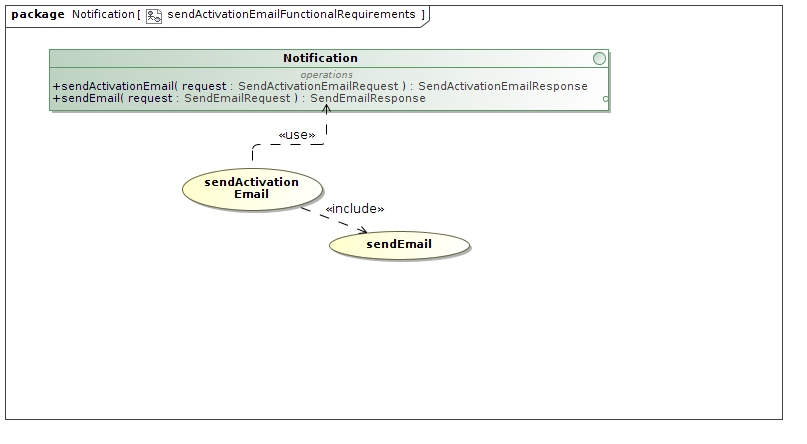
\includegraphics[scale=0.5]{../Diagrams and Charts/Notifications/sendActivationEmailFunctionalRequirements.jpg}
		\caption{The functional requirements for the sendActivationEmail use case}
		\label{sendActivationEmailFunctionalRequirements}
	\end{center}	
\end{figure}

This services makes use of the sendEmail service to actually send the email after
it has performed its bussiness logic.

\subsection{sendPasswordResetMail}
Sends an email to a specific address with a specified heading and content
with the intention resetting the users password, provided all the details 
given are valid.

\subsubsection{Service Contract}
The service contract for the sendPasswordResetMail use case is shown in Figure \ref{sendPasswordResetMailServiceContract}
\begin{figure}[H]
	\begin{center}
		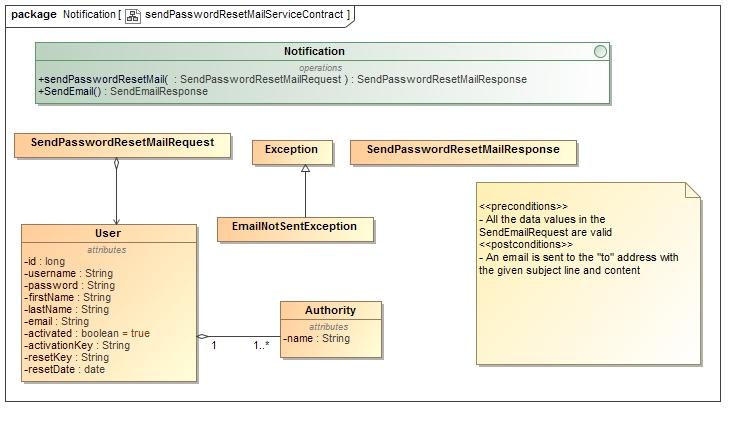
\includegraphics[scale=0.5]{../Diagrams and Charts/Notifications/sendPasswordResetMailServiceContract.jpg}
		\caption{The service contract for the sendPasswordResetMail use case}
		\label{sendPasswordResetMailServiceContract}
	\end{center}
\end{figure}
	
The use case sends an email to a specific address with a specified heading and content
aimed at assisting the user in resetting his/her password, provided all the details
given are valid. If any of the fields in the request object,particularly the "to" field
are not valid the service will throw a EmailNotSentException.

\subsubsection{Functional Requirements}
The lower level services required by the sendPasswordMailReset service to either check the
pre-conditions or address the post-conditions is shown in Figure
\ref{sendPasswordMailFunctionalRequirements}.
\begin{figure}[H]
	\begin{center}
		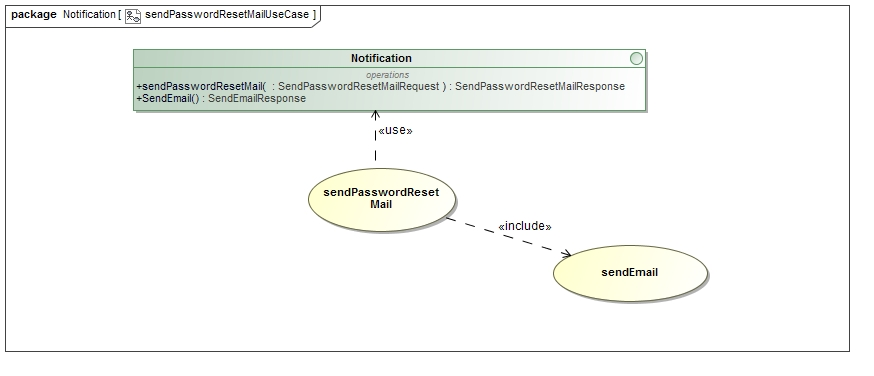
\includegraphics[scale=0.7]{../Diagrams and Charts/Notifications/sendPasswordResetMailUseCase.jpg}
		\caption{The functional requirements for the sendPasswordResetMail use case}
	\end{center}
	\label{sendPasswordMailFunctionalRequirements}
\end{figure}

This services makes use of the sendEmail service to actually send the email after
it has performed its business logic.

\subsection{sendCreationEmail}
Sends an email to a specific address with a specified heading and content
so that the user can activate their account.

\subsubsection{Service Contract}
The service contract for the sendCreationEmail use case is shown in Figure \ref{fig:sendCreationEmailServiceContract}
\begin{figure}[H]
	\begin{center}
		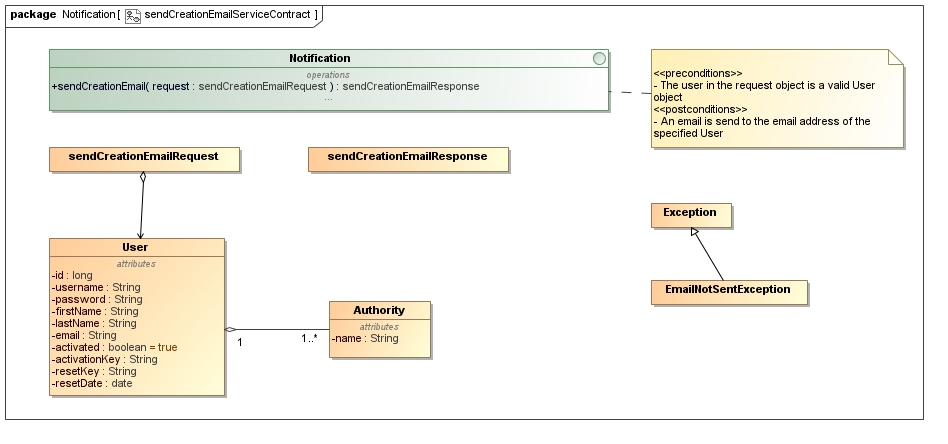
\includegraphics[scale=0.5]{../Diagrams and Charts/Notifications/sendCreationEmailServiceContract.jpg}
		\caption{The service contract for the sendCreationEmail use case}
		\label{sendCreationEmailServiceContract}
	\end{center}
\end{figure}
	
The use case sends an email to a specific address with a specified heading and content
aimed at assisting the user in activating their account, provided all the details
given are valid. If any of the fields in the request object, particularly the "to" field
are not valid the service will throw a EmailNotSentException.

\subsubsection{Functional Requirements}
The lower level services required by the sendCreationEmail service to either check the
pre-conditions or address the post-conditions is shown in Figure
\ref{fig:sendCreationEmailFunctionalRequirements}.
\begin{figure}[H]
	\begin{center}
		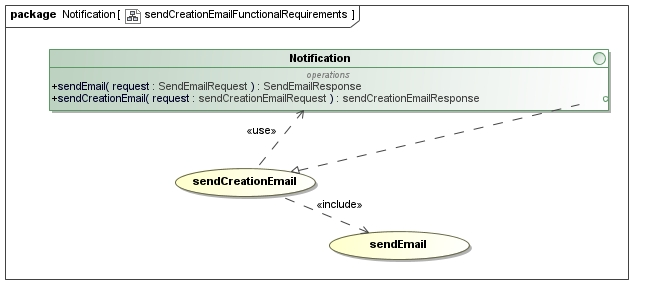
\includegraphics[scale=0.7]{../Diagrams and Charts/Notifications/sendCreationEmailFunctionalRequirements.jpg}
		\caption{The functional requirements for the sendCreationEmail use case}
	\end{center}
	\label{sendCreationEmailFunctionalRequirements}
\end{figure}

This services makes use of the sendEmail service to actually send the email after
it has performed its business logic.



\section{Reporting}
The Reporting Module provides functionality to generate and compare reports
of single/or multiple benchmarks, with the option to export them as csv,
whilst still complying with the quality requirements defined for the system.

\subsection{Architecture Requirements}
\subsubsection{Quality Requirements}
\paragraph*{Flexibility}
The reporting module should be flexible enough to add different elements,
such as graphs, charts and tables. The color scheme should also be easily
changed.

\paragraph*{Performance}
The performance of the reports should as minimalistic as possible, such that the
page is responsive as possible.

\paragraph*{Reliability}
Each report must be reliable with the data it represents, as this is what the
user will be referring to.



\subsection{Architecture Design}
\subsubsection{Architectural Responsibilities, Components and Realization}
The architectural components of the Reporting Module are shown in Figure \ref{fig:reportingResponsibilityAllocation}
\begin{figure}[H]
	\begin{center}
	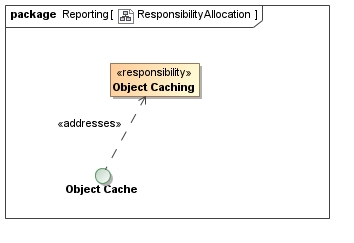
\includegraphics[scale=0.5]{../Diagrams and Charts/Reporting/ResponsibilityAllocation.jpg}
	\caption{The abstract components to which the architectural responsibilities are assigned.}
	\label{fig:reportingResponsibilityAllocation}
	\end{center}
\end{figure}



\subsubsection{Tactics}
The Reporting module should implement the following tactics:
\begin{itemize}
  \item \textit{Report caching} to improve scalability and performance.
\end{itemize}



\subsubsection{Frameworks and Technologies}
The frameworks and technologies used for reporting will consist of JavaScript,
HTML and CSS. With the exporting of reports using a JavaScript library called jsPDF.

We have considered using the jasper reports to generate reports, but it does
 not provide the full functionality that we are looking for. Such as exporting the graphics of the reports.


\section{Test Data}
The \textit{test data} module is responsible for management and cataloguing of
test data to be used in the benchmarking tests.

\subsection{Scope}
The scope for the test data module is shown in Figure \ref{fig:testData}
\begin{figure}[H]
  \begin{center}
  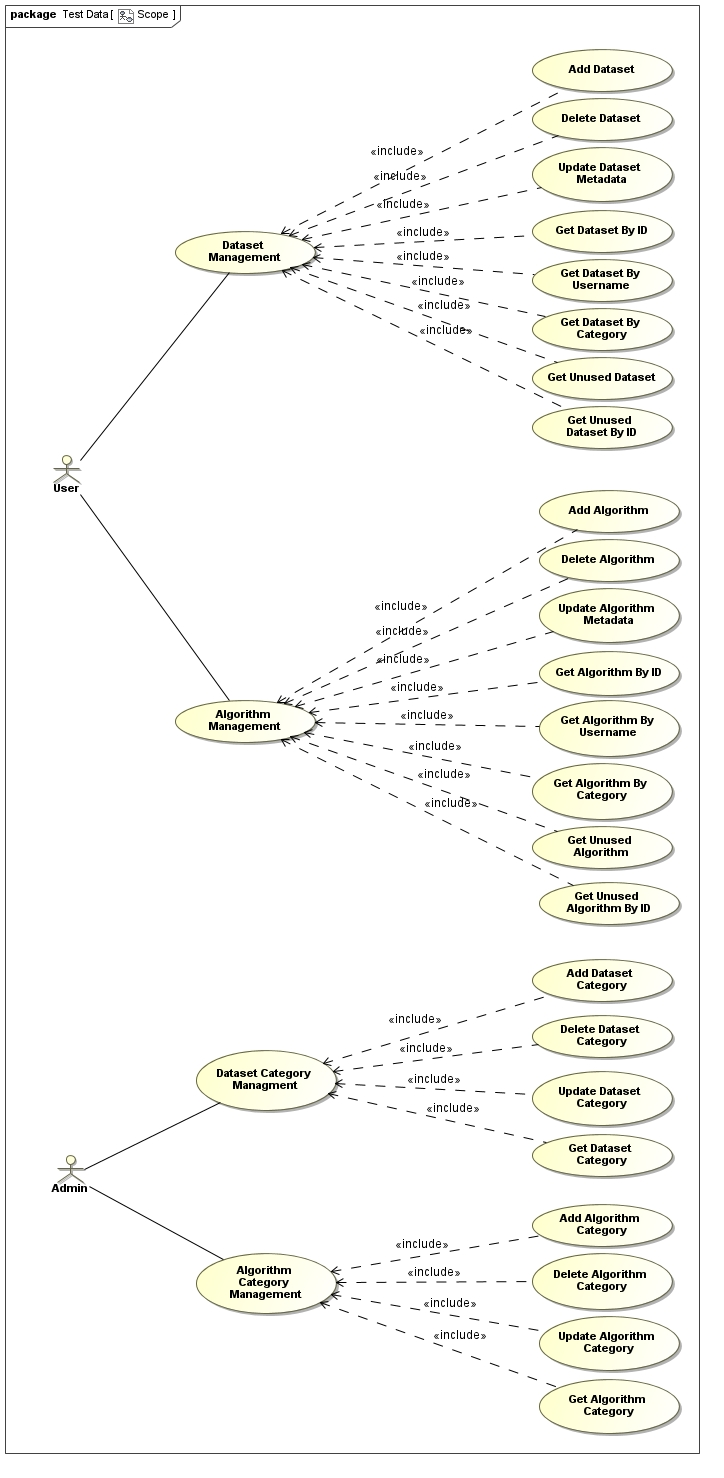
\includegraphics[scale=0.7]{../Diagrams and Charts/Test Data/Scope.jpg}
  \caption{Test Data}
  \end{center}
  \label{fig:testData}
\end{figure}
The scope of the test data module include:
\begin{itemize}
	\item The user can dynamically generate test data
	\item Users can rate dynamic or user upload data sets
	\item Any user can upload there own dataset to the growing repository of data sets 
	\item Users will be able to view the data set with associated meta data
\end{itemize}

\subsection{Domain Model}
The domain model for the test data module is shown in Figure \ref{fig:testDataModel}
\begin{figure}[H]
  \begin{center}
  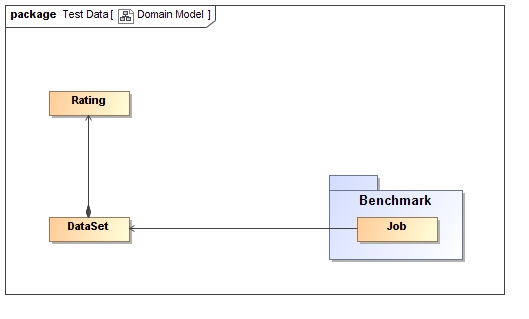
\includegraphics[scale=0.5]{../Diagrams and Charts/Test Data/Domain Model.jpg}  
  \caption{Test Data Domain Model}
  \end{center}
  \label{fig:testDataModel}
\end{figure}


\section{Users}
The \textit{Users} module is responsible for maintaining demographic information
about the registered users of the system, including the Autority levels of each
user.

\subsection{Scope}
The scope for the users module is shown in Figure \ref{Users Scope}
\begin{figure}[H]
  \begin{center}
  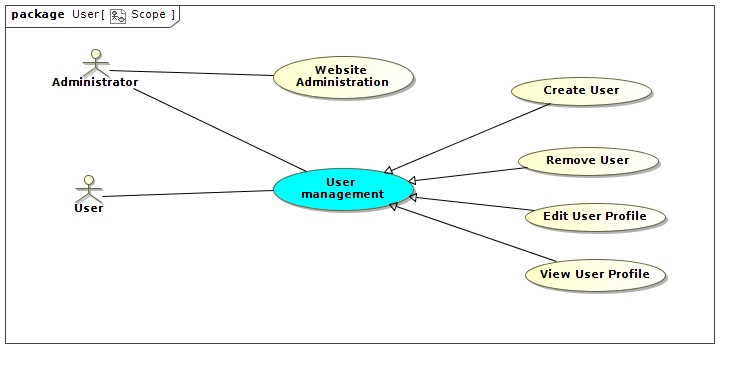
\includegraphics[scale=0.5]{../Diagrams and Charts/Users/Scope.jpg}
  \caption{Users Scope}
  \end{center}
  \label{Users Scope}
\end{figure}
The scope of the users module include:
\begin{itemize}
	\item The Super User can add and remove Administrator users
	\item Administrator users can add and remove Regular Users
	\item Any person who wants use the bechmarking service can add their
	profiles to the system and become a user. They can then also edit or
	remove their profiles
	\item Any user can view the profile of any Administrator or Regular
	user
\end{itemize}

\subsection{Domain Model}
The domain model for the users module is shown in Figure \ref{Users Domain Model}
\begin{figure}[H]
  \begin{center}
  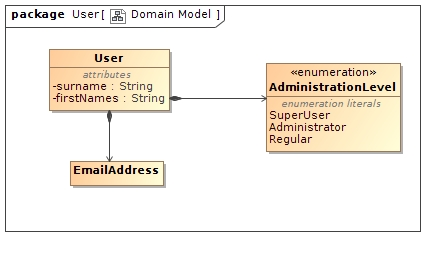
\includegraphics[scale=1.0]{../Diagrams and Charts/Users/Domain Model.jpg}
  \caption{Users Domain Model}
  \end{center}
  \label{Users Domain Model}
\end{figure}
For each user a Surname, First Names and Email Address will be stored.
There are 3 main types of users who
are at different authority levels. There is one and only one "Super User" who
will have full authority over the entire system. Then there are "Administrator"
users who can be assigned or removed by the Super User. The main function of
the Super User is to manage the Administrator users. The Administrator user
wil have the permissions needed to manage the website and to add or remove.
Regular Users if nessesary. Lastly the "Regular Users"
can be created by anyone who wants to use the benchmarking service. These users
will be able to use the service but not do anything administrative.


\end{document}
